\documentclass{article}

\usepackage[letterpaper,margin=1in]{geometry}
\usepackage{graphicx} % Required for inserting images
\usepackage{amsmath}
\usepackage{amsthm}
\usepackage{amssymb}
\usepackage{booktabs}
\usepackage{longtable}
\usepackage{multirow}
\usepackage{mathrsfs}
\usepackage{makecell}
\usepackage{caption}
\usepackage[backend=biber,
style=numeric,
sorting=none
]{biblatex} % If you're using biblatex
\addbibresource{reference.bib}
\usepackage{hyperref}
\usepackage{xurl}
\usepackage{authblk}

\usepackage{placeins}
\usepackage{float}

% \usepackage{siunitx}

\usepackage{relsize}              % in your preamble
\newcommand{\bigveebar}{%
  \mathop{\mathlarger{\mathlarger{\veebar}}}\displaylimits%
}
\newtheorem{proposition}{Proposition}[section]
\newtheorem{theorem}{Theorem}[section]
\newtheorem{corollary}{Corollary}[section]

% Commands used to include orcid (taken from https://gugushvili.github.io/blog/2019/08/09/orcid)
\usepackage{tikz}
\definecolor{lime}{HTML}{A6CE39}
\DeclareRobustCommand{\orcidicon}{
	
\begin{tikzpicture}
	\draw[lime, fill=lime] (0,0) 
	circle [radius=0.16] 
	node[white] {{\fontfamily{qag}\selectfont \tiny ID}};
	\draw[white, fill=white] (-0.0625,0.095) 
	circle [radius=0.007];
	\end{tikzpicture}
	\hspace{-2mm}
}
\foreach \x in {A, ..., Z}{\expandafter\xdef\csname orcid\x\endcsname{\noexpand\href{https://orcid.org/\csname orcidauthor\x\endcsname}
			{\noexpand\orcidicon}}
}
\newcommand{\orcidauthorA}{0000-0002-8308-5016} % For David Bernal
\newcommand{\orcidauthorB}{0000-0002-4474-3266} % For Albert Lee
\newcommand{\orcidauthorC}{0009-0003-8823-8055} % For Woosik Kim


\title{Black-Box Configuration Search for Generalized Disjunctive Programming}
\author[1]{Albert Joon Lee\orcidB}
\author[2]{Woosik Kim\orcidC}
\author[1,*]{David E. Bernal Neira\orcidA}

\affil[1]{Davidson School of Chemical Engineering, Purdue University, West Lafayette, IN 47907, USA}
\affil[2]{Elmore Family School of Electrical and Computer Engineering, Purdue University, West Lafayette, IN 47907, USA}

\date{*Email: dbernaln@purdue.edu}

\begin{document}

\maketitle

\begin{abstract}
Designing chemical processes requires choosing equipment and operating conditions from many alternatives.
Evaluating each design can require costly optimization or simulation.
Generalized disjunctive programming (GDP) links discrete design choices with continuous process variables and the constraints associated with each configuration.
Black-box methods can search these configurations using objective evaluations rather than the full algebraic model.
We compare RBFOpt, Branch-and-Model (BAM), factorization-machine-based optimization with simulated annealing, and a budget-limited discrete steepest descent implementation using stored objective values and separately measured subproblem costs.
The main question is whether higher target attainment under a limited evaluation budget also leads to lower computational cost.
Here we show, across 21 analytical grids and four process GDP benchmark families, that target attainment and computational cost can favor different methods.
BAM achieves the highest grid target attainment at ten evaluations, largely through its initial sampling.
At 100 evaluations, RBFOpt reaches the reference target in 81.9\% of runs compared with 70.0\% for BAM, but its median estimated full-run completion time is higher: 365.74 versus 64.42~s.
For the dynamic process benchmark, RBFOpt reaches the target in all ten runs at a budget of 15 evaluations, whereas discrete steepest descent first does so at the tested budget of 30.
Conventional algebraic methods remain competitive when model expressions and suitable solvers are available.
These comparisons use estimated costs along recorded search paths rather than online solver timings, and support selecting GDP configuration-search methods by considering target attainment, evaluation cost, and search overhead together.
\end{abstract}

\section{Introduction}
In chemical process design, evaluating a single candidate configuration can require a costly optimization or simulation, making the choice of which configuration to explore next a central computational challenge. 
Process design involves discrete decisions, such as equipment selection, the number of processing stages, and operating modes, along with continuous variables such as flow rates, temperatures, and equipment sizes. 
Generalized disjunctive programming (GDP) provides a framework for representing these decisions through Boolean variables, logical propositions, and conditional constraints~\cite{raman1994modelling}. 
In logic-based GDP solution methods, fixing the Boolean variables associated with a selected configuration determines which constraints remain active and yields a reduced optimization subproblem. 
When all discrete decisions are fixed, this subproblem can be formulated as a nonlinear programming (NLP) problem. 
Exploring multiple configurations may therefore require repeatedly solving NLP subproblems, which can be computationally expensive. 
Consequently, identifying high-quality configurations with fewer NLP subproblem evaluations is an important objective in solving GDP problems.

Conventional GDP solution methods generally rely on either mixed-integer nonlinear programming (MINLP) reformulations or logic-based decomposition. 
Big-\(M\) and Hull reformulations transform disjunctive constraints into algebraic formulations~\cite{raman1994modelling,grossmann2003hull}, whereas logic-based approaches select discrete configurations and solve the corresponding reduced subproblems~\cite{turkay1996logic,bergamini2005logic}. 
In logic-based approaches, the strategy used to select discrete configurations can significantly affect the number of subproblem evaluations required.

Our previous work introduced Logic-Based Discrete-Steepest Descent (LD-SDA), which represents ordered Boolean decisions using external integer variables~\cite{ovalle2025logic}. 
LD-SDA explores the resulting integer space through neighborhood search and discrete line search, evaluating selected configurations by solving their corresponding reduced optimization subproblems. 
However, as a local search method, LD-SDA may converge to different locally optimal solutions depending on the starting point and the selected neighborhood.

We compare a budget-limited adaptation of LD-SDA, denoted DSDA, with other derivative-free optimization (DFO) methods for searching the same integer lattice. 
DFO methods use objective evaluations without requiring derivatives with respect to the search variables~\cite{larson2019derivative}. 
We consider RBFOpt, which uses radial basis function surrogate models~\cite{costa2018rbfopt}, and Branch-and-Model (BAM), which combines domain partitioning with local surrogate models~\cite{ma2023bam}. 
Factorization machines provide another approach for modeling interactions between decision variables~\cite{rendle2010factorization}. 
\textcite{kitai2020designing} combined factorization machines
with quantum annealing in the FMQA framework.
Here we test the classical simulated-annealing variant (FMQA-SA).
We compare these methods to investigate whether they can identify high-quality solutions with fewer configuration evaluations, while accounting for the computational overhead of each search strategy.

Although the number of objective evaluations is an important measure of DFO performance~\cite{more2009benchmarking}, fewer evaluations do not necessarily result in lower computational costs. 
In GDP problems, the cost of evaluating a configuration can vary depending on the NLP subproblem and its feasibility, while DFO methods also require computational effort to select new points. 
Therefore, evaluating these methods requires considering both the number and cost of objective evaluations, as well as the computational overhead of the search algorithms.
The main contributions of this work are summarized as follows:

\begin{itemize}
    \item We compare RBFOpt, BAM, and FMQA-SA with the budget-limited DSDA implementation for searching the integer lattice defined by external variables. Their performance is evaluated using common starting points, evaluation budgets, and target attainment criteria.

    \item We formulate 21 existing two-dimensional benchmark functions as GDP problems and compare the black-box methods with conventional GDP solution methods, including GDPopt and Big-$M$/Hull reformulations. This comparison distinguishes methods that use objective evaluations from those that have access to the complete algebraic formulation.

    \item We evaluate the methods on previously published process GDP problems, including Column, CSTR, Small Batch, and Dynamic GDP~\cite{ovalle2025logic,peng2024dynamic}. These experiments examine how the search strategies perform across different discrete domains and feasible configurations.

    \item We analyze evaluation efficiency and computational cost using absolute cumulative success profiles and time-to-solution estimates. Recorded search trajectories are combined with separately measured fixed-configuration subproblem costs to estimate NLP-inclusive completion times and examine the effects of search overhead and unsuccessful evaluations.
\end{itemize}

\section{Background}

\subsection{Generalized Disjunctive Programming and Fixed-Configuration Evaluation}

GDP represents operating and design alternatives using Boolean variables and associated algebraic constraints~\cite{raman1994modelling}. 
The original continuous variables have domain \(\mathcal X=[\underline{\mathbf x},\overline{\mathbf x}]\subseteq\mathbb R^{n_x}\). The original integer variables have domain \(\mathcal Z=[\underline{\mathbf z},\overline{\mathbf z}]\cap\mathbb Z^{n_z}\). 
Let \(K\) index the disjunctions and \(D_k\) index the disjuncts in disjunction \(k\in K\). 
Each disjunct \(i\in D_k\) has a Boolean variable \(Y_{ik}\).
The GDP formulation is given by
\begin{equation}\label{eqn:gdp.general}
\begin{aligned}
\min_{\mathbf x,\mathbf z,\mathbf Y}\quad & f(\mathbf x,\mathbf z)\\
\text{s.t.}\quad &\mathbf g(\mathbf x,\mathbf z)\leq\mathbf 0,\\
&\bigveebar_{i\in D_k}\left[
\begin{gathered}
Y_{ik}\\
\mathbf h_{ik}(\mathbf x,\mathbf z)\leq\mathbf 0
\end{gathered}\right],\qquad k\in K,\\
&\Omega(\mathbf Y)=\mathrm{True},\\
&\mathbf x\in\mathcal X,\quad\mathbf z\in\mathcal Z,\quad
\mathbf Y\in\{\mathrm{False},\mathrm{True}\}^{n_y}.
\end{aligned}\tag{GDP}
\end{equation}
Here, \(f\) is the objective function, \(\mathbf g\) represents the global constraints, and \(\mathbf h_{ik}\) represents the constraints associated with each disjunct. 
The operator \(\veebar\) requires exactly one disjunct to be selected within each disjunction. 
The logical propositions \(\Omega(\mathbf Y)\) impose additional relationships among the Boolean variables.

Following the external-variable reformulation of \textcite{ovalle2025logic}, each ordered group of \(m_j\) Boolean alternatives is represented by an external integer variable \(\xi_j\in\{1,\ldots,m_j\}\), which identifies the selected alternative.
Let \(n_E\) denote the number of external integer variables and \(\mathcal Y_{\mathrm{logic}}\) the set of Boolean assignments satisfying the exactly-one conditions and \(\Omega(\mathbf Y)\). 
The external-variable lattice and its logically admissible subset are
\begin{equation}\label{eqn:external.lattice}
\begin{aligned}
\mathcal L_E&=\prod_{j=1}^{n_E}\{1,\ldots,m_j\},\\
\mathcal E_{\mathrm{adm}}&=\{\boldsymbol\xi\in\mathcal L_E:
\mathbf Y(\boldsymbol\xi)\in\mathcal Y_{\mathrm{logic}}\}.
\end{aligned}
\end{equation}
For each logically admissible configuration $\boldsymbol\xi$, the corresponding Boolean variables are fixed, yielding the following reduced optimization subproblem:

\begin{equation}\label{eqn:Sub}
\begin{aligned}
\Phi(\boldsymbol\xi)=\inf_{\mathbf x,\mathbf z}\quad &f(\mathbf x,\mathbf z)\\
\text{s.t.}\quad &\mathbf g(\mathbf x,\mathbf z)\leq\mathbf 0,\\
&\mathbf h_{ik}(\mathbf x,\mathbf z)\leq\mathbf 0
\quad\text{for all }(i,k)\text{ with }Y_{ik}(\boldsymbol\xi)=\mathrm{True},\\
&\mathbf x\in\mathcal X,\quad\mathbf z\in\mathcal Z.
\end{aligned}\tag{Sub}
\end{equation}
Here, \(\Phi(\boldsymbol\xi)\) represents the optimal objective value of the reduced subproblem. 
For the benchmark problems considered in this study, fixing the Boolean variables yields an NLP. 
If the reduced subproblem is infeasible, we define \(\Phi(\boldsymbol\xi)=+\infty\).

When the external-variable mapping represents all logically admissible Boolean configurations, the original GDP can be expressed as the following upper-level optimization problem~\cite{ovalle2025logic}:
\begin{equation}\label{eqn:outer.value}
\min_{\boldsymbol\xi\in\mathcal E_{\mathrm{adm}}}\Phi(\boldsymbol\xi).
\end{equation}
A logically admissible configuration may still yield an infeasible reduced subproblem.
In this study, candidate configurations are evaluated using precomputed objective values rather than solving the reduced NLP during the search. 
The NLP evaluation costs are measured separately and used in the computational analysis described in Section~\ref{sec:methodology}.

\subsection{Conventional GDP Solution Approaches}
 
Big-\(M\) and Hull reformulations transform GDP models into mixed-integer nonlinear programming (MINLP) formulations by associating Boolean variables \(Y_{ik}\) with binary variables \(y_{ik}\) and translating logical propositions into algebraic constraints~\cite{raman1994modelling,grossmann2003hull}. 
In the Big-\(M\) reformulation, the disjunctive constraints are expressed as \(\mathbf h_{ik}(\mathbf x,\mathbf z)\leq\mathbf M_{ik}(1-y_{ik})\), where the inequality is applied componentwise. 
The Big-\(M\) values must be sufficiently large to render the corresponding constraints redundant when \(y_{ik}=0\), but excessively large values can weaken the continuous relaxation and cause numerical difficulties.

Hull reformulations introduce disaggregated variables, linking constraints, and bounds scaled by binary indicators~\cite{grossmann2003hull}. 
The disjunctive constraints are imposed on the disaggregated variables when \(y_{ik}=1\), whereas \(y_{ik}=0\) forces these variables to zero, making the corresponding disjunct inactive. 
For convex disjunctive sets, this formulation can provide a stronger continuous relaxation than Big-\(M\), although it introduces additional variables and constraints. 
For nonconvex GDP problems, the Hull reformulation does not guarantee a convex reformulated model or global optimality~\cite{chen2022pyomogdp}.

Logic-based outer approximation (LOA) alternates between a mixed-integer master problem and fixed-configuration NLP subproblems~\cite{turkay1996logic}. 
Under suitable convexity and regularity assumptions, the master problem uses linearization cuts to obtain lower bounds, while feasible NLP subproblem solutions provide upper bounds. 
For nonconvex GDP problems, these linearizations may not provide valid global lower bounds, motivating global logic-based outer approximation (GLOA), which requires globally valid relaxations and subproblem bounds. 
\textcite{bergamini2005logic} developed a GLOA approach for process networks using piecewise under- and overestimators.

GDPopt provides implementations of logic-based methods within Pyomo.GDP~\cite{chen2022pyomogdp,pyomoGDPopt}. 
Its relaxation with integer cuts (RIC) method uses an MILP relaxation to select configurations and adds no-good cuts to exclude evaluated discrete assignments, without generating the successive outer-approximation cuts used by LOA~\cite{pyomoGDPopt}.

LD-SDA is an existing alternative that searches ordered external configurations through improving neighborhood moves and discrete line searches~\cite{ovalle2025logic}. 
It selects the best improving neighbor, continues along the resulting direction while improvement persists, and resumes neighborhood exploration. 
The present work uses this discrete-search structure as a reference and compares other configuration-selection strategies and their computational costs.

\subsection{Derivative-Free Optimization}

Derivative-free optimization (DFO) uses function observations without requiring derivatives of the objective with respect to the search variables~\cite{larson2019derivative}. 
For GDP configuration search, the outer method can be derivative-free even if its evaluation routine uses a derivative-based nonlinear solver. 
Surrogate methods seek to reduce expensive evaluations by fitting models to observed data, with computational cost arising from both oracle calls and model-based candidate selection. 

\subsubsection{RBFOpt}
RBFOpt is an open-source surrogate optimizer for bounded black-box problems, with support for continuous, integer, and categorical variables~\cite{costa2018rbfopt,nannicini2021implementation}. 
Given $N$ observed objective values at external integer configurations \(\boldsymbol\xi^{(1)},\ldots,\boldsymbol\xi^{(N)}\), RBFOpt constructs a surrogate model of the form
\begin{equation}\label{eqn:rbf.surrogate}
\widehat\Phi_N(\boldsymbol\xi)
=\sum_{r=1}^{N}\lambda_r\varphi\!\left(\|\boldsymbol\xi-\boldsymbol\xi^{(r)}\|_2\right)
+p(\boldsymbol\xi),
\end{equation}
where \(\widehat\Phi_N(\boldsymbol\xi)\) approximates the objective value at a candidate configuration \(\boldsymbol\xi\), \(\lambda_r\) are interpolation coefficients determined from the observed values, \(\varphi\) is a radial basis function of the Euclidean distance between configurations, and \(p(\boldsymbol\xi)\) is a polynomial tail depending on the selected kernel.

Candidate selection balances low predicted values against exploration away from evaluated points. 
The metric stochastic response surface method (MSRSM) combines scaled surrogate predictions and distances to existing samples, changing their relative weights during the search~\cite{regis2007stochastic}.  
New oracle observations update the model. 

\subsubsection{Branch-and-Model (BAM)}
Branch-and-Model (BAM) combines domain partitioning with local surrogate construction~\cite{ma2023bam}. 
Evaluated points define boxes, and a potentially optimal selection procedure identifies regions for further modeling and search. 
Within selected boxes, Automatic Learning of Algebraic Models (ALAMO) constructs sparse algebraic models from nearby observations~\cite{cozad2014learning}. 
BARON optimizes these local models to propose candidates, while box-size-based exploration maintains broader coverage~\cite{ma2023bam,bamManual,sahinidis1996baron}. 
Thus, BARON acts on learned surrogates within BAM; it is not solving the original GDP through this interface. 
Its support for integer restrictions permits the configuration domains considered here~\cite{bamManual}.

\subsection{Factorization-Machine-Based Optimization}

A second-order factorization machine (FM) models individual feature effects and pairwise interactions through shared latent parameters~\cite{rendle2010factorization}. 
For a binary encoding \(\mathbf b\in\{0,1\}^{m}\) of an external integer configuration \(\boldsymbol\xi\), the fitted FM surrogate is
\begin{equation}\label{eqn:fm.surrogate}
\widehat\Phi_{\mathrm{FM}}(\mathbf b)
=\beta_0+\sum_{i=1}^{m}\beta_i b_i
+\sum_{i=1}^{m-1}\sum_{j=i+1}^{m}
\langle\mathbf a_i,\mathbf a_j\rangle b_i b_j,
\end{equation}
where \(\widehat\Phi_{\mathrm{FM}}(\mathbf b)\) denotes the predicted training response, \(m\) is the number of binary features, \(\beta_0\) is the intercept, $\beta_i$ is the linear coefficient of \(b_i\), and \(\mathbf a_i\in\mathbb R^r\) is its latent vector of dimension \(r\).
The inner product \(\langle\mathbf a_i,\mathbf a_j\rangle\) determines the pairwise interaction coefficient.
The model parameters are learned from evaluated configurations and their corresponding training responses.

For binary inputs, \(b_i^2=b_i\), so the fitted model is a binary quadratic model. 
Dropping its constant term \(\beta_0\) gives the following quadratic unconstrained binary optimization (QUBO) problem:
\begin{equation}\label{eqn:fm.qubo}
\min_{\mathbf b\in\{0,1\}^{m}}\mathbf b^{\mathsf T}\mathbf Q\mathbf b,
\qquad
Q_{ij}=\begin{cases}
\beta_i,&i=j,\\
\langle\mathbf a_i,\mathbf a_j\rangle,&i<j,\\
0,&i>j.
\end{cases}
\end{equation}
The QUBO describes the learned surrogate, not an exact algebraic reformulation of the GDP. 
Moreover, a binary string need not decode to an in-domain, logically admissible configuration.

The factorization machine with quantum annealing (FMQA) framework combines FM surrogate fitting with annealing-based candidate generation~\cite{kitai2020designing}. 
Starting from observed evaluations, the method fits the FM, samples binary candidates from the resulting quadratic model, and evaluates a selected decoded configuration through the objective oracle before updating the training data. 
In the present experiments, the objective is evaluated using a precomputed lookup oracle rather than solving a fixed-configuration NLP during the search, as described in Section~\ref{sec:methodology}. 

The simulated annealing variant of FMQA (FMQA-SA) uses classical simulated annealing to sample binary candidates from the learned QUBO. 
Temperature-dependent acceptance of uphill moves supports exploration, while gradual cooling favors lower-energy solutions~\cite{kirkpatrick1983optimization}. 
No quantum hardware was used in this study.

\section{Experimental Methods}
\label{sec:methodology}\label{sec:cases}

\subsection{Benchmark problems: analytical Grid-GDP}
\label{sec:grid-gdp-formulation}
We consider 21 two-dimensional analytical functions adapted from the Quantum Hamiltonian Descent benchmark collection~\cite{qhdBenchmarks}. 
Each is sampled at 31 equally spaced values per coordinate, giving 961 configurations. 
For each benchmark function, let \([\ell_x,u_x]\) and \([\ell_y,u_y]\) denote the coordinate bounds, and let \(I=J=\{0,\ldots,30\}\) be the corresponding index sets.
The physical coordinates are defined as
\begin{equation}\label{eqn:grid-coordinates}
a_i=\ell_x+\frac{i(u_x-\ell_x)}{30},\qquad
b_j=\ell_y+\frac{j(u_y-\ell_y)}{30}.
\end{equation}

Let \(f\) denote the original analytical objective function, and let \(L\) and \(U\) be its minimum and maximum over the \(31\times31\) lattice.
Both constants are obtained by exhaustive preprocessing of all 961 lattice points before any search.
Each benchmark function is represented by the following GDP:
\begin{equation}\label{eqn:grid-gdp}
\begin{aligned}
\min_{x,y,Y^x,Y^y}\quad & F(x,y)=\frac{f(x,y)-L}{U-L}\\
\mathrm{s.t.}\quad &
\bigvee_{i\in I}\left[\begin{array}{c}Y_i^x\\x=a_i\end{array}\right],\qquad
\bigvee_{j\in J}\left[\begin{array}{c}Y_j^y\\y=b_j\end{array}\right],\\
&\operatorname{ExactlyOne}(Y_0^x,\ldots,Y_{30}^x),\\
&\operatorname{ExactlyOne}(Y_0^y,\ldots,Y_{30}^y),\\
&\ell_x\leq x\leq u_x,\qquad \ell_y\leq y\leq u_y,\\
&Y_i^x,Y_j^y\in\{\mathrm{False},\mathrm{True}\}.
\end{aligned}
\end{equation}
The two exclusive disjunctions contain 62 coordinate-selection Boolean indicators.
The objective retains the analytical expression; it is not a 961-entry lookup-table objective.
Consequently, the algebraic solvers receive the expression and its disjunctive structure, whereas the DFO methods observe only objective values returned at their selected coordinates.

Figure~\ref{fig:grid_gdp_illustration} shows the discrete Rosenbrock objective landscape.
The historical Rosenbrock instance uses
\begin{equation}\label{eqn:grid-rosenbrock}
f(x,y)=(1-x)^2+100(y-x^2)^2,\qquad
x\in[-2,2],\quad y\in[-1,3].
\end{equation}
On this lattice, $L=13/2025$ and \(U=2509\) in exact arithmetic.
Thus \(a_i=-2+2i/15\), \(b_j=-1+2j/15\), and the normalized analytical objective is
\begin{equation}\label{eqn:grid-rosenbrock-normalized}
F(x,y)=\frac{(1-x)^2+100(y-x^2)^2-13/2025}{2509-13/2025}.
\end{equation}
The two exactly-one disjunctions in Equation~\eqref{eqn:grid-gdp} select indices \(i\) and \(j\), fixing \(x=a_i\) and \(y=b_j\); the analytical Rosenbrock objective is then evaluated at that point.
The two minimizers have indices \((22,14)\) and \((23,16)\), corresponding respectively to \((x,y)=(14/15,13/15)\) and \((16/15,17/15)\).

Fixing both coordinate disjunctions fixes \(x\) and \(y\), leaving no remaining original continuous degrees of freedom.
Thus the measured fixed-point GAMS/IPOPT calls characterize fresh model preparation, solver invocation, and verification, rather than a difficult continuous optimization subproblem.
The unfixed analytical objectives remain nonlinear and generally nonconvex, so Big-$M$ and Hull produce MINLP representations.
The complete analytical definitions and coordinate domains of the 21 benchmark functions are provided in the Supplementary Material~\cite{rbfoptTestArchive,qhdBenchmarks}.

\begin{figure}[tbp]
\centering
\includegraphics[width=0.70\textwidth]{figures/grid_rosenbrock_landscape.pdf}
\caption{Discrete Rosenbrock objective landscape on the $31\times31$ grid without interpolation. Colors use $\log_{10}(1+F/10^{-5})$ spacing, with colorbar labels reporting the normalized objective $F$. White diamonds mark the two lattice minimizers.}
\label{fig:grid_gdp_illustration}
\end{figure}

\FloatBarrier

\subsection{Process GDP benchmark problems}
\label{sec:process-cases}
The process benchmarks are the CSTR network, 17-stage distillation column, and Small Batch models of \textcite{ovalle2025logic}, and the nine-stage nonlinear mode-switching model of \textcite{peng2024dynamic}.
Their objectives minimize total reactor volume (CSTR), condenser and reboiler duties plus active tray cost (Column), investment cost (Small Batch), and the negative integral of squared state (Dynamic).
The external variables represent the reactor/feed cutoff and recycle location (CSTR), reflux and boilup positions (Column), parallel unit counts (Small Batch), and final stages of modes 1 and 2 (Dynamic).
The CSTR superstructure contains \(N\) potential reactor positions, where \(N\in\{5,10,15,20,25,30\}\).
Dynamic uses 30 finite elements per stage and three Radau collocation points.
The reference configurations in external variable coordinates are $(N,N)$ for CSTR, \((13,4)\) for Column (physical trays \((14,5)\)), \((2,2,1)\) for Small Batch, and \((1,4)\) for Dynamic.
The cited publications provide the full formulations.

Table~\ref{tab:process-cases} summarizes the original GDP and DFO candidate domains, IPOPT-accepted lookup coverage, measured evaluation coverage, and evaluation budgets.
The process searches use frozen objective tables from fixed-configuration GAMS/IPOPT evaluations; only accepted finite objectives enter the lookup oracle.
Measured coverage includes all configurations in each DFO candidate box, including unsuccessful and structural-rejection evaluations.
The evaluation budget $B$ limits the total number of objective evaluations, including initialization, repeated calls, and infeasible evaluations.
The full GDP box precedes logical and algebraic feasibility restrictions.
Column searches \(\{7,\ldots,15\}\times\{1,\ldots,9\}\) (81 coordinates) within its original \(\{1,\ldots,15\}^{2}\) box (225 coordinates); other cases use their full boxes.
For CSTR, recycle/feed ordering admits \(N(N+1)/2\) logical candidates; this does not imply that every candidate produces an accepted IPOPT solution.
Dynamic permits \(z_{E,1}<z_{E,2}\) or \((z_{E,1},z_{E,2})=(9,9)\).

Small Batch uses all 27 configurations in \(\{1,2,3\}^{3}\), whose decisions count parallel mixer, reactor, and centrifuge units.
Of these configurations, 15 are rejected during feasibility-based bound tightening (FBBT) preprocessing.

\begin{table}[htbp]
\centering
\caption{Process GDP domains, IPOPT-accepted lookup coverage, measured point-cost coverage, evaluation budgets, and reference objective values.}
\label{tab:process-cases}
\footnotesize
\setlength{\tabcolsep}{4pt}

\textbf{(a) External-variable domains}\par\smallskip
\begin{tabular}{@{}lllrr@{}}
\toprule
Model & Full GDP box & DFO candidate box &
\makecell{Full GDP\\box size} &
\makecell{DFO\\box size} \\
\midrule
Column & \(\{1,\ldots,15\}^{2}\) &
\(\{7,\ldots,15\}\times\{1,\ldots,9\}\) & 225 & 81 \\
CSTR \(N\) & \(\{1,\ldots,N\}^{2}\) &
\(\{1,\ldots,N\}^{2}\) & \(N^2\) & \(N^2\) \\
Small Batch & \(\{1,2,3\}^{3}\) &
\(\{1,2,3\}^{3}\) & 27 & 27 \\
Dynamic & \(\{1,\ldots,9\}\times\{2,\ldots,9\}\) &
\(\{1,\ldots,9\}\times\{2,\ldots,9\}\) & 72 & 72 \\
\bottomrule
\end{tabular}

\par\medskip
\textbf{(b) Lookup coverage and evaluation budgets}\par\smallskip
\begin{tabular}{@{}lrrrr@{}}
\toprule
Model &
\makecell{Finite\\lookup} &
\makecell{Measured\\coordinates} &
\makecell{Evaluation\\budget $(B)$} &
\(f_{\mathrm{ref}}\) \\
\midrule
Column & 29 & 81 & 16 & 19346.1248 \\
CSTR 5 & 15 & 25 & 8 & 3.0620146 \\
CSTR 10 & 54 & 100 & 15 & 2.8895370 \\
CSTR 15 & 120 & 225 & 22 & 2.8293941 \\
CSTR 20 & 210 & 400 & 29 & 2.7994064 \\
CSTR 25 & 325 & 625 & 36 & 2.7814826 \\
CSTR 30 & 458 & 900 & 43 & 2.7695697 \\
Small Batch & 12 & 27 & 10 & 167427.6571 \\
Dynamic & 37 & 72 & \makecell{12,15,20,\\30,37,50} & -212.0088 \\
\bottomrule
\end{tabular}
\end{table}
\FloatBarrier

\subsection{Search protocol and compared algorithms}

\subsubsection{Shared initialization and evaluation budgets}
Each Grid-GDP benchmark uses ten initial designs and evaluation budgets \(B\in\{10,30,50,70,100\}\). Across four methods, this gives \(21\times10\times5\times4=4{,}200\) DFO runs.
The process benchmarks comprise 140 paired conditions per method, totaling 560 runs (Table~\ref{tab:process-cases}).
For each condition, three distinct initial configurations are generated using seeded Latin hypercube sampling, mapped to integer coordinates, and shared in the same order across all four methods.
All process cases use seeds 0--9, with no replacement of failed starts. Column seed 0 has three unaccepted initial configurations; the resulting DSDA execution failure remains in the ten-run denominator.

Methods may terminate before exhausting the evaluation budget \(B\).
Internal cache accesses without objective callbacks are not counted as evaluations.
Feasibility and target attainment are determined from the original lookup values rather than method-specific penalties.
For the CSTR reruns, unaccepted evaluations return $+\infty$ to DSDA and RBFOpt; for Column, Dynamic, and Small Batch, those two methods use $10^6$. BAM receives \texttt{NaN} in all process cases. FMQA-SA retains infinite raw values and separately reports $10^6$. These penalties do not replace the recorded solver status or establish mathematical infeasibility.

\subsubsection{Budget-limited LD-SDA-based search (DSDA)}
DSDA is the budget-limited implementation used in this study, adapting the neighborhood search and discrete line search of the published LD-SDA method to the external integer lattice~\cite{ovalle2025logic}.
It evaluates the unit $L_\infty$ neighborhood in fixed enumeration order, selects the best improving neighbor, and continues along the resulting direction through discrete line search.
An improvement requires an objective decrease greater than $10^{-12}$, with ties resolved by the first enumerated neighbor.
Neighborhood exploration resumes from the last improving point.
If the evaluation budget $B$ is exhausted, the best solution found is retained.

For the process benchmarks, DSDA starts from the best feasible configuration among the three evaluated initial points.
For Grid-GDP benchmarks, initial configurations are ranked by objective value, and successive descents are attempted until the evaluation budget is exhausted or the stored target is reached within an absolute tolerance of $10^{-12}$.
For all process benchmarks, DSDA searches within the declared integer bounds without precomputed feasibility filtering.
Infeasible and repeated objective evaluations count toward the evaluation budget.
Unaccepted evaluations return $+\infty$ for CSTR and $10^6$ for the other process cases.

\subsubsection{RBFOpt}
RBFOpt uses MSRSM with automatic RBF selection and solver-based global search~\cite{costa2018rbfopt,nannicini2021implementation}. 
The RBF setting is \texttt{rbf=auto}; the \texttt{global\_search\_method} option is set to \texttt{solver}.
All external variables are treated as integers, and the three shared initial configurations are supplied for evaluation with RBFOpt's additional initialization strategy disabled.
Bonmin solves the auxiliary surrogate MINLPs used for candidate selection, while IPOPT is configured for auxiliary NLPs.
These auxiliary solver calls contribute to the optimizer runtime but do not count toward the objective evaluation budget.
Unaccepted evaluations return $+\infty$ for CSTR and $10^6$ for the other process cases.

\subsubsection{BAM}
BAM uses local algebraic surrogate models optimized by BARON to generate candidate configurations~\cite{ma2023bam,bamManual}.
All external variables are specified as integers using \texttt{integrality=1}.
The three shared initial configurations are evaluated and supplied through \texttt{x\_evaluated} and \texttt{f\_evaluated}, with no additional starting point (\texttt{x0=None}).
The remaining evaluation budget is set to \texttt{max\_evals}=$B-3$, while other algorithmic settings retain their defaults.
Unaccepted evaluations in the process benchmarks return \texttt{NaN}.
Objective evaluations, including repeated calls, are counted independently by the external ledger. For the process experiments, callback $B$ returns its value normally and BAM terminates through its native evaluation limit. All 140 BAM runs use this corrected stopping procedure with the original paired seeds and frozen IPOPT tables; no selection between old and new outcomes is made.

\subsubsection{FMQA-SA}
FMQA-SA uses the PyTorch-based FM implementation from the \texttt{QHD\_Data} branch of \nolinkurl{SECQUOIA/bbo_via_fmqa}~\cite{secquoiaBboFmqa}.
At each adaptive iteration, a second-order rank-eight FM with identity activation is initialized with linear and latent weights drawn from a normal distribution with mean zero and standard deviation $0.01$, and zero bias.
The model is trained on all previously evaluated configurations for 1,000 full-batch epochs using Adam, mean squared error, and a learning rate of $0.01$ on CPU in \texttt{float32}.
Observed finite objective values are min--max scaled to $[0,1]$ (or zero when all finite values are identical), while non-finite evaluations receive a training target of $2.0$.
For reporting and incumbent tracking, non-finite raw objective values are represented by $10^6$.

Each external integer coordinate $\xi_j$ is encoded in unsigned binary using $\lfloor\log_2 u_j\rfloor+1$ bits, where $u_j>0$ is its upper bound.
The fitted FM is converted to a QUBO, with its coefficients scaled by the maximum absolute entry of the quadratic matrix.
Binary candidates are generated using D-Wave's classical \texttt{SimulatedAnnealingSampler} with 100 reads, 1,000 sweeps, and a geometric inverse-temperature schedule~\cite{kirkpatrick1983optimization}.
The lowest-energy decoded candidate within coordinate bounds that has not previously been evaluated is selected; if none is available, a candidate is drawn uniformly from the remaining unevaluated configurations.
GDP logical constraints and NLP feasibility are not screened before oracle evaluation, so infeasible configurations may still consume the evaluation budget.
The new observation is appended, and FM fitting and candidate generation repeat until the evaluation budget $B$ or the 1,800~s method time limit is reached.

\subsection{Execution environment and algebraic comparisons}
\label{sec:protocol}
All computational experiments were conducted on the Dantzig server, equipped with an AMD EPYC 7643 processor (48 cores, 2.3~GHz) and 1~TB RAM.
All optimization methods and numerical libraries were configured for single-threaded execution.
The software environment included Pyomo 6.10.0, GAMS 52.2, RBFOpt 4.3.0, BAM 5.0.0, PyTorch 2.8.0, BARON 25.11.17, and HiGHS 1.12.0.

\paragraph{DFO benchmarking.}
DSDA, RBFOpt, BAM, and FMQA-SA were executed using lookup-based objective evaluations under the initialization and evaluation-budget protocols described in Section~\ref{sec:grid-gdp-formulation} and the preceding subsections.
The objective evaluations were recorded separately from the computational time required by each optimization method.

\paragraph{Fixed-disjunction NLP evaluations.}
To measure the computational cost of evaluating individual configurations, the Boolean decisions of the original GDP formulations were fixed, and the resulting continuous subproblems were evaluated using GAMS/IPOPT with MUMPS.
For the Grid-GDP benchmarks, all 20,181 configurations were evaluated individually, while the process benchmarks used fixed-configuration evaluations of the corresponding process models.
IPOPT used a tolerance of \(10^{-8}\) and a 60~s solver time limit per configuration.
The process oracle accepts finite objectives only when the configured termination and primal-feasibility checks pass; failed solves remain unaccepted rather than being declared globally infeasible.
CSTR sizes 5--25 use the mass-balance/zero-recycle initialization, whereas CSTR30 retains constructor defaults. Column uses the saved 17-tray initialization, and Dynamic uses fresh clones of the unsolved discretized template.
These process-NLP settings are separate from the auxiliary surrogate solvers used inside the DFO methods.
These measurements were conducted independently of the DFO searches and used for the computational cost estimates described in Section~\ref{sec:cost-accounting}.

\paragraph{Algebraic GDP comparisons.}
The conventional comparisons include GDPopt RIC, GLOA, and LOA, as well as Big-\(M\) and Hull reformulations.
GDPopt uses HiGHS for MILP master problems and BARON for nonlinear subproblems~\cite{chen2022pyomogdp,pyomoGDPopt}.
The Big-\(M\) and Hull reformulations are solved using BARON as the MINLP solver.
All algebraic methods use the original GDP domains, a time limit of 1,800~s per instance, and a relative optimality gap of \(10^{-5}\).

\subsection{Target attainment and cumulative success profiles}
\label{sec:metrics}
Let $f_{\mathrm{best}}$ denote the best feasible lookup objective value observed so far and $f_{\mathrm{ref}}$ the reference objective value.
A run reaches the reference target when
\begin{equation}\label{eqn:target}
 |f_{\mathrm{best}}-f_{\mathrm{ref}}|
 \leq 10^{-5}\max\{1,|f_{\mathrm{ref}}|\}.
\end{equation}
Target attainment measures agreement with the reference value rather than certifying global optimality.
For the process reruns, $f_{\mathrm{ref}}$ is the minimum accepted objective in the frozen IPOPT table, and execution failures count as non-successes even if a target was observed earlier.
The hard budget wrapper records callback $B$ before stopping the search. BAM returns this value and stops through its native limit; the other process methods retain the wrapper stop, so their terminal value is observed but not returned to the optimizer. Twenty of the 291 successful process runs first observe the target at callback $B$: six BAM observations are returned and 14 observations from the other methods are not.
For the full-process-GDP comparison, a feasible objective at or below $f_{\mathrm{ref}}+10^{-5}\max\{1,|f_{\mathrm{ref}}|\}$ counts as attainment, so solutions better than the reference are also included.

For each evaluation budget $B$, let $\mathcal R_B$ denote the set of problem--seed instances compared across methods, and let $s$ identify a solution method.
For each instance $r\in\mathcal R_B$, $H_{sBr}$ equals one if the run reaches the target and zero otherwise.
Let $E_{sBr}$ be the index of the first objective evaluation at which the target is reached, with $E_{sBr}=+\infty$ if the target is not reached.
At a threshold of $N$ objective evaluations, where $0\leq N\leq B$, the absolute evaluation-count profile is
\begin{equation}\label{eqn:absolute-evaluations}
 C^{\mathrm{eval}}_{sB}(N)
 =\frac{1}{|\mathcal R_B|}\sum_{r\in\mathcal R_B}
 \mathbf{1}\{H_{sBr}=1,\ E_{sBr}\leq N\}.
\end{equation}
Here, $\mathbf{1}\{\cdot\}$ equals one when the stated conditions hold and zero otherwise, and $|\mathcal R_B|$ is the number of problem--seed instances.
Thus, $C^{\mathrm{eval}}_{sB}(N)$ gives the fraction of runs that reach the target within $N$ evaluations.
For the Grid-GDP benchmarks, $|\mathcal R_B|=210$ at each budget; for each process benchmark and budget, $|\mathcal R_B|=10$.
All runs, including target misses, remain in the denominator.

Let $\widehat T_{sBr}$ denote the estimated full-run completion time calculated as described in Section~\ref{sec:cost-accounting}.
For a time threshold $t\geq0$, measured in seconds, the absolute completion-time profile is
\begin{equation}\label{eqn:absolute-time}
 C^{\mathrm{time}}_{sB}(t)
 =\frac{1}{|\mathcal R_B|}\sum_{r\in\mathcal R_B}
 \mathbf{1}\{H_{sBr}=1,\ \widehat T_{sBr}\leq t\}.
\end{equation}
This profile gives the fraction of runs that reach the target and have an estimated full-run completion time no greater than $t$.
A successful run is counted at its full completion estimate, not at the time of its first target attainment.

Experiments at different evaluation budgets are analyzed separately; a larger-budget trajectory need not extend a smaller-budget trajectory.
Both profiles use absolute evaluation counts or times rather than solver-relative cost ratios~\cite{dolan2002benchmarking}.
The evaluation-count profile is related to data profiles~\cite{more2009benchmarking}, but uses raw rather than dimension-normalized evaluation counts.
Algebraic results are reported separately because their iterations and subsolver calls are not DFO objective evaluations, and only one run is reported for each problem--method pair.

\subsection{Runtime accounting and restart estimates}
\label{sec:cost-accounting}
For a recorded lookup-based run with $n$ objective evaluations and measured lookup-call times, the estimated full-run completion time is
\begin{equation}\label{eqn:reconstructed-cost}
 \widehat T_{\mathrm{complete}}
 =T_{\mathrm{recorded}}-\sum_{q=1}^{n}t_q^{\mathrm{lookup}}
  +\sum_{q=1}^{n}c(\boldsymbol\xi^{(q)})+t_{\mathrm{prep}}.
\end{equation}
Here, $T_{\mathrm{recorded}}$ is the measured runtime of the lookup-based search, $t_q^{\mathrm{lookup}}$ is the measured lookup-processing interval of its $q$th objective call, and $\boldsymbol\xi^{(q)}$ is the external integer configuration evaluated in that call. For the process reruns, this interval covers coordinate processing and in-memory lookup, but excludes callback-file writing; the CSV is loaded before the search clock starts.
The point cost $c(\boldsymbol\xi^{(q)})$ is measured separately for the same benchmark model, problem size, and configuration, including configuration-specific preparation, preprocessing, solver invocation when required, and validation.
The term $t_{\mathrm{prep}}$ accounts for one-time model preparation not already included in the point costs.
The retained search time includes surrogate fitting, candidate generation, auxiliary optimization, and recording performed within the method clock.
Every recorded objective call contributes its point cost, including initialization, repeated visits, and preprocessing rejections; the same stored measurement is used each time a configuration is revisited.

\paragraph{Grid-GDP timers.}
Grid-GDP enumeration and objective normalization are excluded from the timing analysis, and $t_{\mathrm{prep}}=0$ because configuration-specific preparation is included in the point costs.
For DSDA on the Grid-GDP benchmarks, lookup-call times were not recorded, so the method runtime is retained without subtracting lookup time.

\paragraph{Process timers.}
Each original recorded point cost is preserved with its objective and status. Separately measured rejection costs complete the previously unmeasured structural exclusions: 435 for CSTR30, 17 for Column, and 35 for Dynamic.
These coordinates follow the same model preparation and logical-rejection paths, with no NLP solver invocation. Their positive total processing times are measured rather than set to zero.
No cross-size CSTR timing substitution or successful-retry selection is used.
For Dynamic, the original model-template construction and discretization cost is included once per run through $t_{\mathrm{prep}}$; additional campaign-level preparation is not charged repeatedly.
All in-budget evaluations have measured point costs, and all 560 process runs have complete reconstructed completion estimates. The sole execution failure, a Column DSDA initialization failure, retains its recorded cost and contributes zero target success.
These estimates retain the recorded lookup trajectories rather than measuring online optimizer--NLP executions.

Algebraic GDP completion times are measured separately and are not augmented with the DFO point costs.
Grid-GDP algebraic timings include per-run preparation, reformulation, solution, and validation, but exclude shared-template preparation and lattice enumeration.
Full-process-GDP timings include model-template preparation.

\paragraph{Independent-restart estimate.}
For each problem, method, and evaluation budget, let $n_{\mathrm{rep}}=10$ denote the number of runs and $h$ the number reaching the reference target.
The empirical success fraction is $\widehat p=h/n_{\mathrm{rep}}$.
Let $\widetilde T$ denote the median estimated full-run completion time across all $n_{\mathrm{rep}}$ runs, including target misses.
For a per-run success probability $p$, let $R_{99}(p)$ denote the total number of independent runs required to achieve at least a 99\% probability of reaching the target at least once.
The estimated time to solution at this success probability is
\begin{equation}\label{eqn:tts}
 \widehat{\mathrm{TTS}}_{99}
 =\widetilde T\,R_{99}(\widehat p),\qquad
 R_{99}(p)=
 \begin{cases}
 \left\lceil\ln(0.01)/\ln(1-p)\right\rceil,&0<p<1,\\
 1,&p=1,\\
 \infty,&p=0.
 \end{cases}
\end{equation}
Here, $\lceil\cdot\rceil$ denotes rounding up to the nearest integer.
The calculation assumes independent restarts, substitutes the observed success fraction for the unknown success probability, and uses $\widetilde T$ as the representative cost of each run.
With ten observations, it is an empirical restart estimate rather than a statistical guarantee of 99\% success.
The median TTS99 across the 21 Grid-GDP benchmark functions includes infinite estimates.
TTS99 is not calculated for the algebraic methods, which have only one run per problem--method pair.

\section{Computational Results and Discussion}
\label{sec:results}

\subsection{Search Performance on Analytical Grid-GDP Benchmarks}
\label{sec:grid-search-results}
The evaluation budget changes the observed ordering of the four methods (Table~\ref{tab:grid-hits}).
At ten evaluations, BAM reaches the reference target in 111 of 210 problem--seed runs (52.9\%), compared with 45 (21.4\%) for RBFOpt.
Of BAM's 111 successes, 11 occur during shared initialization and 100 at two predetermined Sobol sampling points (10 at a corner and 90 at the grid center), before surrogate-guided candidate selection.
At all tested evaluation budgets from 30 onward, RBFOpt achieves the highest aggregate target-hit fraction, reaching 172 of 210 runs (81.9\%) at 100 evaluations, compared with 147 (70.0\%) for BAM.
These results highlight the importance of initial sampling in low-budget optimization.

\begin{table}[htbp]
\centering
\caption{Grid-GDP reference-target hit percentages from the recorded trajectories. Each cell contains 210 runs (21 functions and ten seeds). The evaluation budget includes the three shared initial evaluations, and repeated objective callbacks are counted toward the evaluation budget.}
\label{tab:grid-hits}
\begin{tabular}{rrrrr}\toprule
Budget $B$ & DSDA & RBFOpt & BAM & FMQA-SA\\\midrule
10 & 6.2 & 21.4 & 52.9 & 7.6\\
30 & 35.7 & 63.3 & 54.8 & 22.4\\
50 & 42.4 & 71.9 & 57.6 & 36.2\\
70 & 48.1 & 76.2 & 62.9 & 48.6\\
100 & 49.5 & 81.9 & 70.0 & 61.4\\
\bottomrule
\end{tabular}
\end{table}

Figure~\ref{fig:grid-profiles} shows the cumulative fraction of runs attaining the reference target as a function of the number of objective evaluations, revealing when successful searches first reach the target.
Each panel is a separate budget experiment, so trajectories at a larger evaluation budget are not assumed to extend those at a smaller evaluation budget.
DSDA attains more targets than FMQA-SA at evaluation budgets of 30 and 50, whereas their aggregate attainment is nearly identical at an evaluation budget of 70 (101 versus 102 successful runs). 
At the largest tested evaluation budget of 100, FMQA-SA reaches 129 targets compared with 104 for DSDA. 

\begin{figure}[htbp]
\centering\includegraphics[width=\linewidth]{figures/figure_B_grid_evaluation_profiles.pdf}
\caption{Absolute evaluation-count cumulative success profiles for the four DFO methods. The horizontal axis is the number of objective callbacks to first target attainment; the vertical axis is the fraction of all 210 problem--seed instances reaching the target within that count. Initial and repeated callbacks count, unsuccessful runs remain in the denominator, and counts are not normalized by another solver. The panels use evaluation budgets of 10, 30, 50, 70, and 100.}
\label{fig:grid-profiles}
\end{figure}

\FloatBarrier

\subsection{Computational Comparison on Grid-GDP Problems}
\label{sec:grid-gdp-results}
The analytical formulation in Section~\ref{sec:grid-gdp-formulation} permits comparison with algebraic methods and a specified fixed-point evaluation protocol.
Completion estimates for 4,200 DFO runs attach individually measured GAMS/IPOPT costs for all 20,181 grid coordinates to the 201,833 recorded callbacks.
Every actual callback, including a repeated visit, receives the cost of its coordinate under the accounting rules in Section~\ref{sec:cost-accounting}.

The fixed-point measurements have mean and median costs of 0.6522 and 0.3727~s, respectively; the mean is higher because some external solver calls incur long delays.
Because both coordinates are fixed, the measured point costs primarily reflect the fixed-configuration evaluation protocol, including solver-interface and evaluation overhead, rather than the solution of an NLP with free continuous decision variables.
At $B=100$, RBFOpt reaches more targets than BAM but has a substantially higher median completion estimate: 365.74 versus 64.42~s (Table~\ref{tab:grid-cost}).
Their median summed point costs are similar, at 61.21 and 63.97~s, while their median retained search components are 306.98 and 0.430~s.
The additional target coverage therefore comes with substantial optimizer overhead; its value depends on the required coverage and the relative costs of configuration evaluation and candidate selection.
FMQA-SA's 62.04~s median search component is comparable to its 62.34~s median summed point cost, contributing to a 124.13~s median completion estimate.
DSDA has a small retained search component (approximately 0.0032~s) and can terminate below the evaluation budget, giving a median completion estimate of 24.14~s alongside its lower target coverage.
The medians of separate cost components need not sum to the median total.

\begin{table}[htbp]
\centering
\caption{Grid-GDP DFO results at an evaluation budget of $B=100$. Each method has 210 runs. Completion and summed point-cost medians include target hits and misses; they are not first-hit times or TTS99 estimates.}
\label{tab:grid-cost}
\begin{tabular}{lrrr}\toprule
Method & Target hits & Median completion (s) & Median point cost (s)\\\midrule
DSDA & 104/210 & 24.14 & 24.14\\
RBFOpt & 172/210 & 365.74 & 61.21\\
BAM & 147/210 & 64.42 & 63.97\\
FMQA-SA & 129/210 & 124.13 & 62.34\\
\bottomrule
\end{tabular}
\end{table}

Figure~\ref{fig:tts99} combines empirical hit rates with median full-run completion costs under the independent-restart assumption.
At $B=100$, the medians of the 21 problem-specific TTS99 estimates are 194.10~s for DSDA, 948.42~s for RBFOpt, 84.77~s for BAM, and 757.81~s for FMQA-SA, retaining infinite values.
DSDA and BAM nevertheless have zero observed hits on four and two functions, respectively; RBFOpt and FMQA-SA have at least one hit on every function at that evaluation budget.
BAM's lower median TTS99 therefore reflects favorable restart-cost estimates for the typical benchmark function, but does not account for its unresolved zero-hit cases.
For applications requiring coverage across heterogeneous problems, the infinity counts are as relevant as the median; for a known problem, its own hit rate and completion cost are more informative than the suite median.
Because the empirical hit probabilities are estimated from only ten seeds per function, these TTS99 values should be interpreted as descriptive median-cost restart proxies rather than measured 99\% solution-time guarantees.

Table~\ref{tab:grid-gdp-outcomes} reports the algebraic solver results separately because their iterations and subsolver calls are not equivalent to DFO callbacks and one selected run is included per problem and method.
The algebraic solver families and configurations are described in Section~\ref{sec:protocol}.
Each GDPopt method---RIC, GLOA, and LOA---attains the reference target on 18 of 21 functions; all three miss H\"older table, Michalewicz, and the historical modified Shubert instance.
Target attainment can coexist with termination at a time limit, as in the three Camel3 cases and the Levy13/RIC run.
Consequently, the measured completion time of a target-attaining run must be distinguished from a completed global-optimality certification.

Big-\(M\)/BARON attains four of 21 targets and Hull/BARON five of 21.
Each has 16 unsupported functions because the configured GAMS/BARON interface does not accept the required sine/cosine expressions.
These entries are solver-compatibility limitations, not optimization timeouts or mathematical failures of either reformulation.
Among the five supported functions, target-attaining runs have measured worker completion times between approximately 0.55 and 1.30~s; Hull attains all five targets, whereas Big-\(M\) misses Styblinski--Tang.
The ten executed target misses are marked F, even when the raw solver termination is optimal; unsupported cases are marked U and remain in the denominator.
Only the 63 target-attaining runs receive numerical times in the table, while all failed-run times are retained in the source records.
For example, the target-attaining Rosenbrock runs complete in 0.758~s with Big-\(M\) and 0.813~s with Hull.
These supported cases demonstrate that access to the algebraic structure can be highly competitive, while the full-suite hit fractions additionally reflect implementation coverage.

\begin{figure}[htbp]
\centering\includegraphics[width=\linewidth]{figures/figure_C_grid_completion_profiles.pdf}
\caption{Absolute completion-time cumulative success profiles for Grid-GDP. The horizontal axis is estimated full-run completion time in seconds on a logarithmic scale; the vertical axis is the fraction of all 210 problem--seed instances that reached the target and completed within that time. Estimates combine recorded search overhead with the sum of measured fixed-point GAMS/IPOPT costs along the complete recorded path. Misses retain their finite completion estimates in the run data but contribute no success. These are neither first-hit-time curves nor solver-relative ratios. GDPopt and reformulations are excluded.}
\label{fig:grid-completion-profiles}
\end{figure}

\begin{figure}[htbp]
\centering\includegraphics[width=\linewidth]{figures/figure_D_grid_tts99.pdf}
\caption{Estimated Grid-GDP TTS99 in seconds on a logarithmic vertical axis. Method groups are DSDA (blue), RBFOpt (orange), BAM (green), and FMQA-SA (purple). Within each method, adjacent groups use budgets 10, 30, 50, 70, and 100, marked by circles, squares, diamonds, triangles, and filled plus signs, respectively. Each finite point represents one function. Black horizontal lines show the budget-specific median over all 21 functions, retaining infinite estimates; an infinite median is labeled above the plot. Annotations $\infty\!\times n$ count functions with no observed target hits at each budget. A low median can therefore coexist with incomplete suite coverage. Estimates follow Equation~\eqref{eqn:tts}, using median estimated full-run costs across all ten seeds, including target misses, and assuming independent restarts. The costs are retrospective fixed-path estimates, not measured online solution times.}
\label{fig:tts99}
\end{figure}

\begin{table}[htbp]
\centering
\caption{Target attainment and measured completion times for the selected Grid-GDP runs. Each cell represents one run for one problem and method. Numerical entries are measured full-worker completion times in seconds for target-attaining runs only; they are not times to first target attainment. Target attainment does not certify global optimality.}
\label{tab:grid-gdp-outcomes}
\small
\setlength{\tabcolsep}{4pt}
\renewcommand{\arraystretch}{1.13}
\begin{tabular}{@{}lrrrrr@{}}
\toprule
Problem & \shortstack{GDPopt\\RIC} & \shortstack{GDPopt\\GLOA} & \shortstack{GDPopt\\LOA} & \shortstack{Big-M/\\BARON} & \shortstack{Hull/\\BARON} \\
\midrule
Ackley & 899.10 & 909.69 & 310.47 & U & U \\
Alpine 1 & 0.88 & 0.85 & 0.95\textsuperscript{*} & U & U \\
Alpine 2 & 1789.14\textsuperscript{T} & 1789.40\textsuperscript{T} & 1795.11\textsuperscript{T} & U & U \\
Bohachevsky 2 & 175.17 & 223.44 & 154.58 & U & U \\
Three-hump camel & 1800.10\textsuperscript{T*} & 1789.34\textsuperscript{T*} & 1789.64\textsuperscript{T*} & 1.15 & 1.00 \\
Csendes & 0.92 & 0.94 & 1.21 & U & U \\
Deflected corrugated spring & 507.80 & 440.76 & 378.11 & U & U \\
Drop-Wave & 120.15\textsuperscript{*} & 176.69\textsuperscript{*} & 221.96\textsuperscript{*} & U & U \\
Easom & 1176.78 & 1769.44 & 1787.95 & U & U \\
Griewank & 1214.84 & 1581.92 & 1042.31 & U & U \\
Holder Table & \textbf{F} & \textbf{F} & \textbf{F} & U & U \\
Hosaki & 1569.06 & 1524.42 & 1758.69 & 1.30 & 1.29 \\
Levy & 1731.14 & 1746.53 & 1794.67\textsuperscript{T} & U & U \\
Levy 13 & 1800.10\textsuperscript{T} & 1789.92\textsuperscript{T} & 1774.92 & U & U \\
Michalewicz & \textbf{F} & \textbf{F} & \textbf{F} & U & U \\
Rastrigin & 78.26 & 114.81 & 180.11 & U & U \\
Rosenbrock & 334.94 & 278.13 & 655.39 & 0.76 & 0.81 \\
Shubert & \textbf{F} & \textbf{F} & \textbf{F} & U & U \\
Styblinski-Tang & 1339.67 & 1440.10 & 1562.35 & \textbf{F} & 0.95 \\
Sum of squares & 822.85\textsuperscript{*} & 754.81\textsuperscript{*} & 851.15\textsuperscript{*} & 0.55 & 0.58 \\
Xin-She Yang 3 & 1.01 & 0.90 & 1.37 & U & U \\
\midrule
Target hits / all problems & 18/21 & 18/21 & 18/21 & 4/21 & 5/21 \\
Executed target misses & 3 & 3 & 3 & 1 & 0 \\
Unsupported & 0 & 0 & 0 & 16 & 16 \\
\bottomrule
\end{tabular}
\par\vspace{5pt}
\begin{minipage}{\linewidth}
\footnotesize
F: an executed run that did not attain the reference target, including runs whose raw solver termination is optimal. U: unsupported expression; these cases remain in the denominator of 21 problems per method.\par
T: termination at a time limit. A target-attaining run retains its numerical time and T marker. *: runs from the \texttt{pyomo610-grid-v1} execution profile; these ten selected runs are distinct from the ten target misses marked F.\par
Worker times include worker-side preparation, transformation, solve, and validation, and exclude shared-template preparation and lattice enumeration. The source records retain failed-run times, raw solver statuses, termination information, objectives, archive identifiers, and hashes.\par
\end{minipage}
\end{table}
\FloatBarrier

\subsection{Process GDP Case Studies}
\label{sec:process-results}
The following computational results are based on the process GDP benchmark problems previously investigated in the LD-SDA studies.

\subsubsection{Target attainment on the recorded lookup paths}
The process reruns use IPOPT-generated objective tables and ten paired seeds per condition. All evaluations within the declared bounds, including structural rejections, failed evaluations, and repeated calls, count toward the evaluation budget.
Across the 560 runs, 291 reach the target, 268 miss it, and one fails during execution; the failure remains in the denominator (Table~\ref{tab:process-targets}).

RBFOpt reaches the CSTR target in 59 of 60 runs across the six size-dependent budgets, compared with 15 for DSDA, 18 for BAM, and nine for FMQA-SA.
At CSTR30 and $B=43$, RBFOpt reaches all ten targets, DSDA three, BAM two, and FMQA-SA one.
These results favor RBFOpt under the tested budgets, although model size and budget increase together.

For Column, DSDA reaches five targets, RBFOpt and FMQA-SA four each, and BAM none.
All methods use the restricted 81-configuration box. The failed DSDA run with three unaccepted initial points is retained rather than replaced by a different seed.
Small Batch uses all 27 configurations. At $B=10$, DSDA reaches eight targets, FMQA-SA six, RBFOpt five, and BAM two. Of the 400 callbacks, 196 are rejected during preprocessing.

For Dynamic, RBFOpt reaches nine targets at $B=12$ and all ten from $B=15$ onward. DSDA reaches all ten from $B=30$ onward.
BAM reaches four targets at $B=30$, seven at $B=37$, and all ten at $B=50$. FMQA-SA reaches six targets at $B=50$.
All 140 BAM runs terminate at their declared evaluation limits, with no budget-control failures. A callback-level comparison with the initial executions confirms identical configurations, accepted objectives, and point costs for all 3,430 BAM evaluations. Changes in success counts arise from corrected execution classification, rather than changed search paths.

\begin{table}[htbp]
\centering
\caption{Reference-target attainment in the IPOPT-table process experiments. Entries are audited target hits divided by all ten paired seeds at evaluation budget $B$.}
\label{tab:process-targets}
\small
\begin{tabular}{@{}lrcccc@{}}
\toprule
Case & $B$ & DSDA & RBFOpt & BAM & FMQA-SA \\
\midrule
Column & 16 & 5/10\textsuperscript{F1} & 4/10 & 0/10 & 4/10 \\
CSTR 5 & 8 & 2/10 & 10/10 & 10/10 & 3/10 \\
CSTR 10 & 15 & 2/10 & 10/10 & 1/10 & 2/10 \\
CSTR 15 & 22 & 2/10 & 10/10 & 1/10 & 1/10 \\
CSTR 20 & 29 & 3/10 & 9/10 & 2/10 & 1/10 \\
CSTR 25 & 36 & 3/10 & 10/10 & 2/10 & 1/10 \\
CSTR 30 & 43 & 3/10 & 10/10 & 2/10 & 1/10 \\
Small Batch & 10 & 8/10 & 5/10 & 2/10 & 6/10 \\
Dynamic & 12 & 4/10 & 9/10 & 0/10 & 2/10 \\
Dynamic & 15 & 5/10 & 10/10 & 3/10 & 3/10 \\
Dynamic & 20 & 8/10 & 10/10 & 3/10 & 3/10 \\
Dynamic & 30 & 10/10 & 10/10 & 4/10 & 4/10 \\
Dynamic & 37 & 10/10 & 10/10 & 7/10 & 5/10 \\
Dynamic & 50 & 10/10 & 10/10 & 10/10 & 6/10 \\
\bottomrule
\end{tabular}
\par\vspace{3pt}
\begin{minipage}{0.96\linewidth}
\footnotesize Superscript F$n$ denotes $n$ execution failures, which remain in the denominator and do not count as hits. The only failure is a Column DSDA initialization failure. All 56 groups use seeds 0--9. All BAM slots were rerun with corrected stopping and the same inputs and seeds; the other methods retain their original runs. A target observation at callback $B$ counts; BAM returns that value, while the other methods stop in the wrapper. The reference is the accepted IPOPT-table minimum, not a global-optimality certificate.
\end{minipage}
\end{table}

Figure~\ref{fig:process-evaluations} shows the first target-attaining evaluation on successful recorded runs, with misses and execution failures retained in the denominator.
\begin{figure}[htbp]
\centering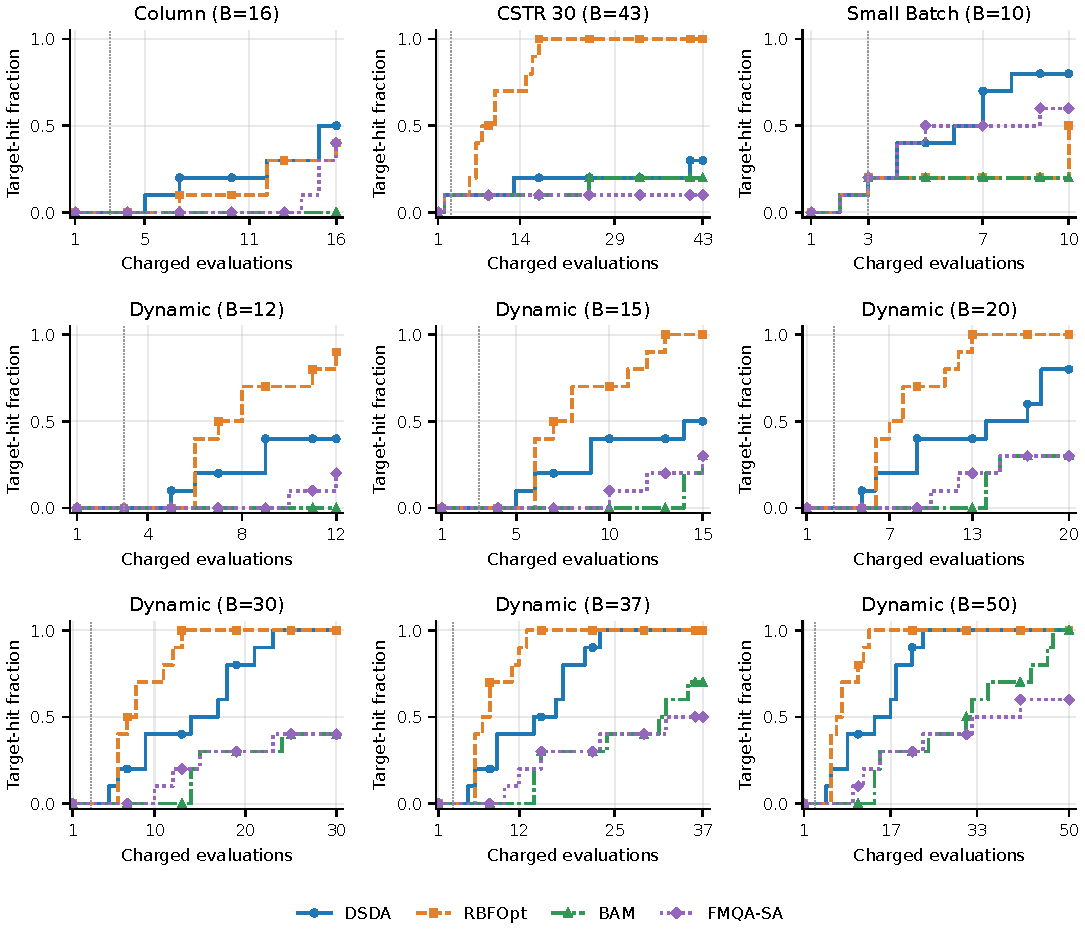
\includegraphics[width=\linewidth]{figures/process_evaluation_profiles.pdf}
\caption{Cumulative audited target attainment versus charged evaluations for nine illustrative process conditions. Every method--condition group retains all ten seeds, including execution failures. Initialization, unsuccessful evaluations, and repeated callbacks consume the budget. The first target observation on a successful run determines each step, including a terminal observation at callback $B$. Line styles and markers distinguish methods. All 14 conditions appear in Table~\ref{tab:process-targets}.}
\label{fig:process-evaluations}
\end{figure}

\subsubsection{All-outcome NLP costs and objective consistency}
The complete process cost tables cover 2,455 case/size/coordinate keys across the nine models. The 12,822 in-budget callbacks visit 1,790 distinct keys: 1,030 with accepted solutions, 745 rejected by logical checks or preprocessing, and 15 without an accepted solver solution.
All recorded callbacks are within budget. The corrected BAM runs contain neither out-of-budget requests nor missing terminal records, so complete-run cost estimates are available for every seed.

The original 10,070 CSV-backed callbacks agree exactly with their frozen input rows in accepted status, objective, and recorded point cost; 8,255 of these callbacks return accepted finite objectives.
The other 2,752 in-budget callbacks are structural exclusions whose processing costs are now supplied by separate measurements for the same model and size. All in-budget callbacks therefore have measured point costs, including every repeated visit.
The Column and Dynamic full-box measurements also reproduce the original accepted flags and accepted objective values exactly on their 64 and 37 overlapping coordinates. Original overlapping point costs are retained; only previously missing structural-rejection costs are added.
Using the IPOPT tables consistently removes the earlier pairing of BARON lookup objectives with incompatible selected IPOPT results. This establishes consistency of the frozen oracle and cost records, not global optimality or measured online optimizer--NLP performance.

Figure~\ref{fig:nlp-cost} separates optimizer/search overhead from point-evaluation and one-time preparation costs for four illustrative conditions.
For RBFOpt, the search share is 6.82\% for Column, 16.68\% for Small Batch, 39.27\% for CSTR30, and 78.74\% for Dynamic at $B=50$.
DSDA's search share is below 0.2\% in these four conditions. The component includes all operations retained within the method clock after subtracting measured lookup-processing time, rather than isolated surrogate-solving time.
Dynamic DSDA executes 221 callbacks across ten $B=50$ runs, compared with 500 for each of RBFOpt, BAM, and FMQA-SA. Its lower cost reflects shorter paths as well as low search overhead; unsuccessful candidates are evaluated and charged within the common box.

\begin{figure}[htbp]
\centering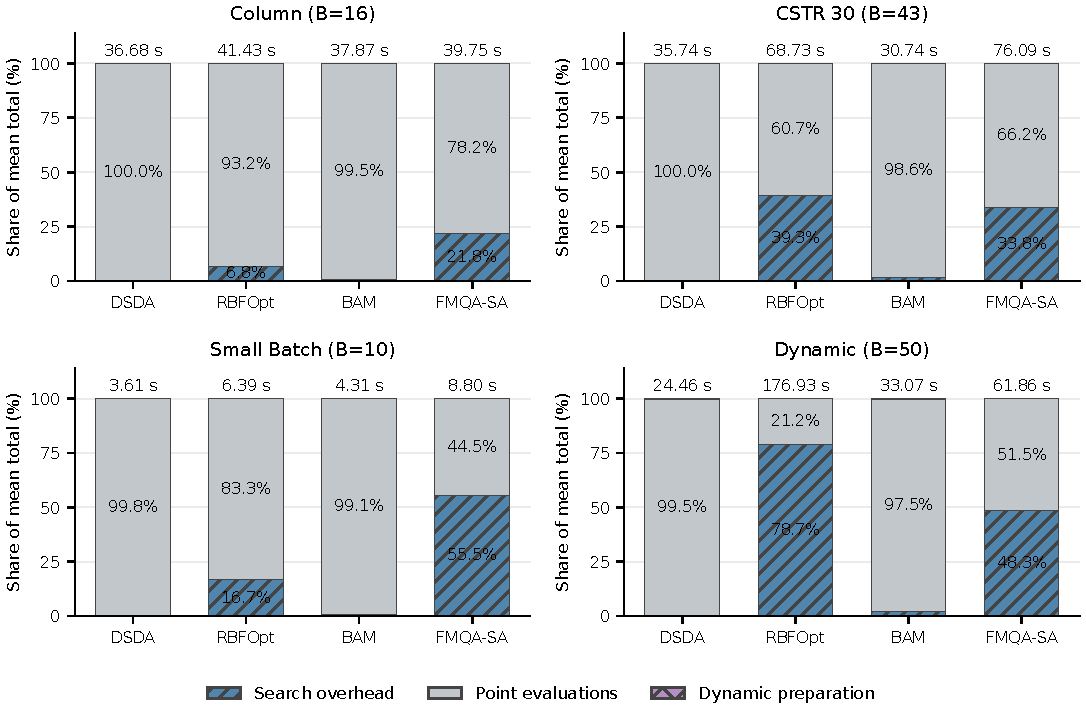
\includegraphics[width=\linewidth]{figures/process_cost_breakdown.pdf}
\caption{Relative computational costs for four process conditions. Each bar uses all ten seeds, including target misses; shares are $100\overline{T}_k/\overline{T}_{\mathrm{total}}$, and numbers above bars give mean reconstructed seconds. Hatching denotes search overhead, gray denotes point evaluations, and crosshatching denotes one-time Dynamic preparation. Shares below 5\% are unlabeled. Every in-budget repeated or unsuccessful evaluation is charged. Structural-rejection costs are measured, original point costs are preserved, and no selected-retry or cross-size cost substitution is used.}
\label{fig:nlp-cost}
\end{figure}

\subsubsection{Absolute completion profiles and restart estimates}
Figure~\ref{fig:process-completion} presents audited target attainment against reconstructed full-run completion time for the same nine illustrative conditions.
For Dynamic at $B=30$, DSDA and RBFOpt both reach ten targets, with median completion estimates of 26.61 and 51.09~s, respectively.
RBFOpt already reaches all ten at $B=15$ with a median of 18.08~s. Thus the comparison depends on whether the evaluation budget is fixed or selected separately for each method.

\begin{figure}[htbp]
\centering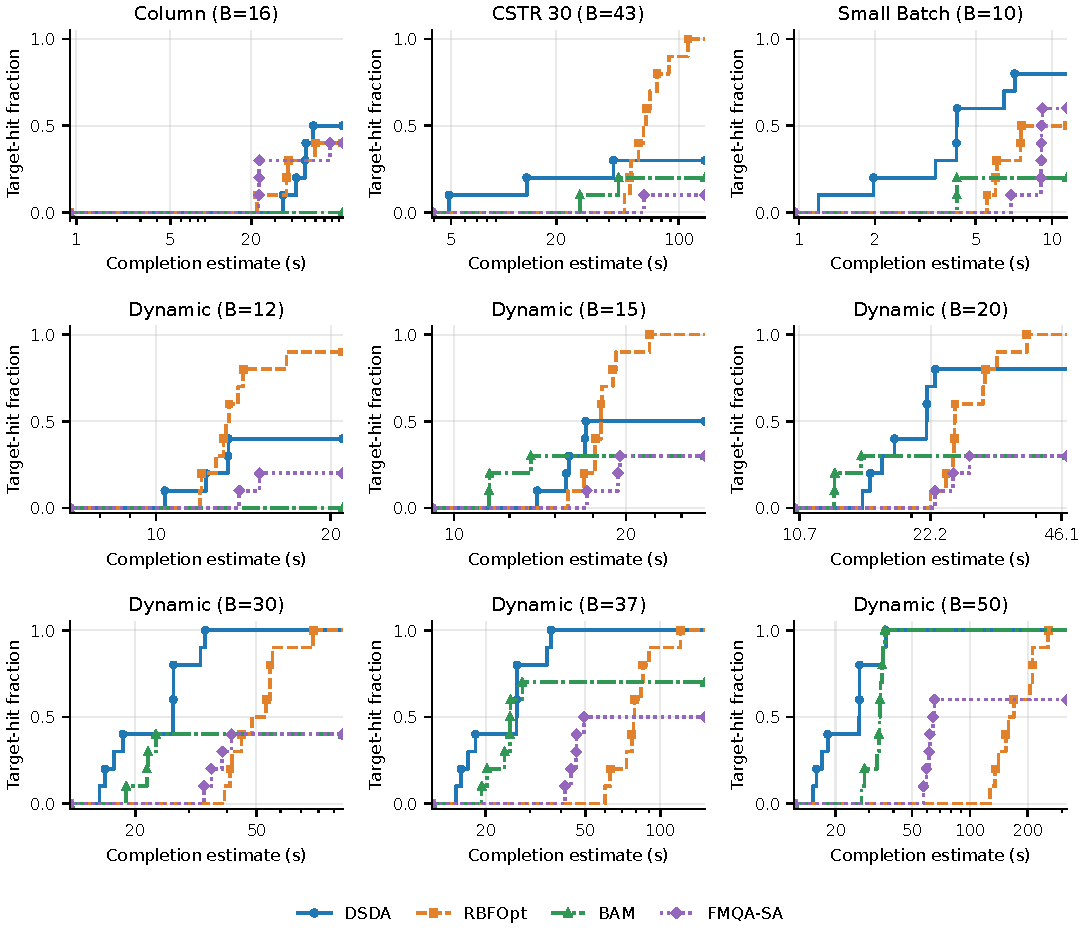
\includegraphics[width=\linewidth]{figures/process_completion_profiles.pdf}
\caption{Absolute cumulative target-attainment profiles for nine process conditions. The horizontal axis is reconstructed full-run completion time on a logarithmic scale; all ten seeds remain in each denominator. Only successful runs contribute steps. Target misses and execution failures contribute no success. Every run has a complete cost estimate. These are fixed-path estimates, not first-hit-time curves or solver-relative ratios. All 14 conditions are summarized in Table~\ref{tab:process-tts99}.}
\label{fig:process-completion}
\end{figure}

Table~\ref{tab:process-tts99} reports all-ten-run completion medians and empirical TTS99 values for all 14 conditions.
Of the 56 groups, 54 have finite TTS99 estimates. The two zero-hit BAM groups, Column at $B=16$ and Dynamic at $B=12$, have infinite estimates; no group has missing timing data.
For CSTR30, RBFOpt has a TTS99 of 64.27~s, compared with 506.21~s for DSDA and 621.30~s for BAM, despite lower median completion costs for DSDA and BAM (38.94 and 29.59~s, respectively).
At Dynamic $B=50$, all three methods reach ten targets; BAM's TTS99 is 33.98~s, between DSDA's 26.60~s and RBFOpt's 164.01~s.
For Small Batch, DSDA has the lowest TTS99 at 11.50~s, followed by RBFOpt at 42.13~s.
These estimates combine empirical success fractions with complete-run medians and do not provide statistical 99\% guarantees.

Figure~\ref{fig:process-scatter} shows the variation among individual timed runs, distinguishing hits, misses, and execution failures.
\begin{figure}[htbp]
\centering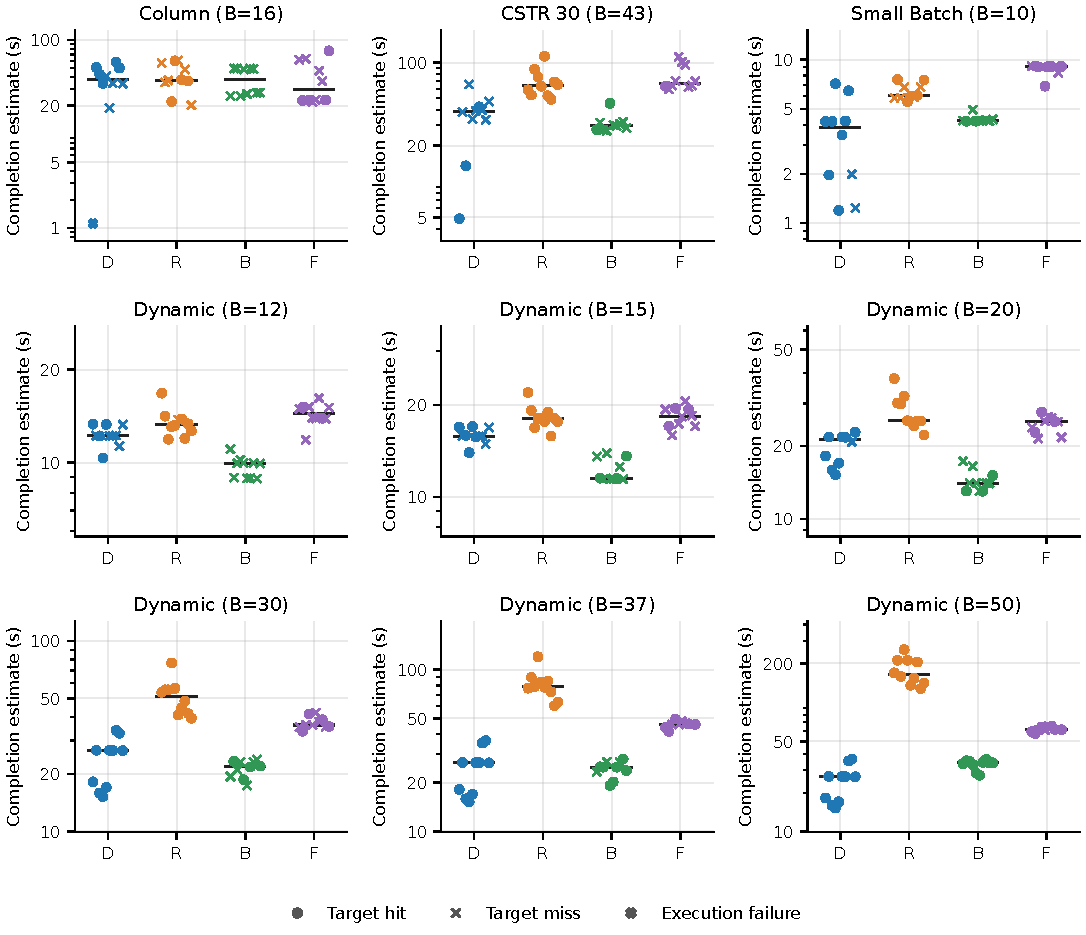
\includegraphics[width=\linewidth]{figures/process_completion_scatter.pdf}
\caption{Individual reconstructed completion times for nine process conditions. D, R, B, and F denote DSDA, RBFOpt, BAM, and FMQA-SA. Circles denote target hits, crosses target misses, and filled crosses timed execution failures; horizontal offsets follow seed order. Black lines are medians over all ten seeds, whose completion costs are available in every group. Misses retain finite costs. These points are neither first-target times nor TTS99 estimates.}
\label{fig:process-scatter}
\end{figure}

\begin{table}[htbp]
\centering
\caption{Median reconstructed completion seconds (empirical TTS99 seconds) for all 14 process conditions. Medians use all ten seeds, including misses and timed execution failures.}
\label{tab:process-tts99}
\small
\setlength{\tabcolsep}{3pt}
\begin{tabular}{@{}lrcccc@{}}
\toprule
Case & $B$ & DSDA & RBFOpt & BAM & FMQA-SA \\
\midrule
Column & 16 & 37.91 (265.36) & 37.35 (373.55) & 37.97 (\(\infty\)) & 29.72 (297.25) \\
CSTR 5 & 8 & 10.66 (223.89) & 11.01 (11.01) & 10.67 (10.67) & 13.92 (180.98) \\
CSTR 10 & 15 & 20.98 (440.66) & 22.17 (22.17) & 18.54 (815.87) & 27.07 (568.40) \\
CSTR 15 & 22 & 29.92 (628.31) & 35.02 (35.02) & 27.67 (1217.37) & 42.82 (1883.92) \\
CSTR 20 & 29 & 40.67 (528.71) & 52.57 (105.15) & 39.37 (826.80) & 59.10 (2600.34) \\
CSTR 25 & 36 & 51.67 (671.73) & 72.73 (72.73) & 50.47 (1059.97) & 74.70 (3286.67) \\
CSTR 30 & 43 & 38.94 (506.21) & 64.27 (64.27) & 29.59 (621.30) & 66.79 (2938.80) \\
Small Batch & 10 & 3.83 (11.50) & 6.02 (42.13) & 4.23 (88.88) & 9.09 (54.57) \\
Dynamic & 12 & 12.22 (122.17) & 13.28 (26.56) & 9.95 (\(\infty\)) & 14.47 (303.79) \\
Dynamic & 15 & 15.84 (110.87) & 18.08 (18.08) & 11.53 (149.85) & 18.39 (239.11) \\
Dynamic & 20 & 21.29 (63.87) & 25.45 (25.45) & 14.07 (182.90) & 25.23 (328.03) \\
Dynamic & 30 & 26.61 (26.61) & 51.09 (51.09) & 21.91 (219.08) & 36.24 (362.38) \\
Dynamic & 37 & 26.60 (26.60) & 78.41 (78.41) & 24.99 (99.95) & 46.05 (322.34) \\
Dynamic & 50 & 26.60 (26.60) & 164.01 (164.01) & 33.98 (33.98) & 61.31 (367.89) \\
\bottomrule
\end{tabular}
\par\vspace{3pt}
\begin{minipage}{0.96\linewidth}
\footnotesize TTS99 follows Equation~\eqref{eqn:tts}, using unrounded ten-seed medians. Infinity denotes zero audited hits. Every group has a complete all-ten-run completion median. All in-budget point costs and lookup-processing times are available; none is zero-filled or borrowed across CSTR sizes. The estimates are retrospective fixed-path costs, not measured online times or 99\% guarantees.
\end{minipage}
\end{table}

\FloatBarrier


Table~\ref{tab:full-gdp} compares five algebraic methods on nine process GDP models.
All 45 saved solutions satisfy the original GDP constraints within a tolerance of $10^{-5}$.
The target-attainment counts are 3/9 for RIC, 1/9 for GLOA, 4/9 for LOA, 7/9 for Big-$M$, and 6/9 for Hull.
These single-run results do not establish success probabilities or global optimality.

All five methods attain the Small Batch reference.
Big-$M$ and Hull complete in 0.55 and 0.57~s, respectively, compared with median DFO completion estimates ranging from 3.83 to 9.09~s.
This demonstrates the competitiveness of algebraic methods when the formulation is available, although the different information access and timing protocols prevent direct speedup claims.

Solver-reported termination is distinguished from independently checked feasibility and target attainment.
All six CSTR GLOA runs report \texttt{optimal}, but their objectives are worse than the saved RIC solutions that pass the original-GDP feasibility recheck. Relative to the accepted IPOPT references, eight raw \texttt{optimal} reports have worse objectives: these six GLOA runs, Column Big-$M$, and CSTR30 Hull. The returned objectives, completion times, and termination labels are retained; the corresponding optimality claims remain unresolved and are not used as global-optimality certificates.
Some reported BARON lower bounds likewise conflict with better saved feasible solutions. The causes of these discrepancies have not been established, and no specific defect in GDPopt or BARON is inferred from these observations.
Furthermore, LOA finds a CSTR15 objective below the lookup reference but reaches the time limit.
These observations highlight the distinction between target attainment, feasible solutions, and valid global-optimality certificates.

\begin{table}[htbp]
\centering
\caption{Full-process-GDP results: objective (measured completion seconds, including model-template preparation). GDPopt uses BARON for nonlinear subproblems and HiGHS for master problems; Big-$M$ and Hull use BARON.}
\label{tab:full-gdp}
\small
\setlength{\tabcolsep}{3pt}
\begin{tabular}{@{}lccccc@{}}
\toprule
Model & RIC & GLOA & LOA & Big-\(M\) & Hull \\
\midrule
CSTR 5 & \makecell{3.0619840\\(31.27)} & \makecell{3.1301981\({}^{\ddagger}\)\\(3.76)} & \makecell{3.0619840\\(31.82)} & \makecell{3.0620136\\(9.12)} & \makecell{3.0620146\({}^{\dagger}\)\\(14.86)} \\
CSTR 10 & \makecell{2.8895081\\(214.06)} & \makecell{3.4479640\({}^{\ddagger}\)\\(4.56)} & \makecell{2.8895081\\(234.13)} & \makecell{2.8894835\\(123.74)} & \makecell{2.8895358\({}^{\dagger}\)\\(126.47)} \\
CSTR 15 & \makecell{2.9660174\({}^{\mathrm{TL}}\)\\(1798.83)} & \makecell{3.5225520\({}^{\ddagger}\)\\(26.19)} & \makecell{2.8293506\({}^{\mathrm{TL}}\)\\(1799.38)} & \makecell{2.8293940\({}^{\mathrm{TL}}\)\\(1799.00)} & \makecell{2.8293941\({}^{\dagger}\)\\(940.36)} \\
CSTR 20 & \makecell{2.9095042\({}^{\mathrm{TL}}\)\\(1799.04)} & \makecell{3.6161230\({}^{\ddagger}\)\\(6.79)} & \makecell{2.8895081\({}^{\mathrm{TL}}\)\\(1797.72)} & \makecell{2.7994063\({}^{\mathrm{TL}}\)\\(1798.72)} & \makecell{2.7994064\({}^{\mathrm{TL}}\)\\(1797.44)} \\
CSTR 25 & \makecell{2.8594370\({}^{\mathrm{TL}}\)\\(1797.05)} & \makecell{3.6478181\({}^{\ddagger}\)\\(85.20)} & \makecell{2.7951055\({}^{\mathrm{TL}}\)\\(1797.46)} & \makecell{2.7814826\({}^{\mathrm{TL}}\)\\(1797.67)} & \makecell{2.7814826\({}^{\mathrm{TL}}\)\\(1797.41)} \\
CSTR 30 & \makecell{2.8379523\({}^{\mathrm{TL}}\)\\(1792.52)} & \makecell{3.1543081\({}^{\ddagger}\)\\(718.80)} & \makecell{2.7844377\({}^{\mathrm{TL}}\)\\(1798.92)} & \makecell{2.7695698\({}^{\mathrm{TL}}\)\\(1797.31)} & \makecell{2.8093862\({}^{\dagger\ddagger}\)\\(1466.60)} \\
Column & \makecell{22271.549\({}^{\mathrm{TL}}\)\\(1797.54)} & \makecell{22271.549\({}^{\mathrm{TL}}\)\\(1798.15)} & \makecell{22271.549\({}^{\mathrm{TL}}\)\\(1797.77)} & \makecell{19853.723\({}^{\dagger\ddagger}\)\\(34.36)} & \makecell{20837.080\({}^{\mathrm{TL}}\)\\(1797.17)} \\
Dynamic & \makecell{-119.383\({}^{\mathrm{TL}}\)\\(1797.71)} & \makecell{-119.383\({}^{\mathrm{TL}}\)\\(1797.55)} & \makecell{-119.383\({}^{\mathrm{TL}}\)\\(1797.84)} & \makecell{-207.626\({}^{\mathrm{TL}}\)\\(1797.51)} & \makecell{-28.597\({}^{\mathrm{TL}}\)\\(1797.77)} \\
Small Batch & \makecell{167427.657\\(12.86)} & \makecell{167427.657\\(14.49)} & \makecell{167427.657\\(5.11)} & \makecell{167427.657\\(0.55)} & \makecell{167427.657\\(0.57)} \\
\bottomrule
\end{tabular}
\par\vspace{3pt}
\begin{minipage}{0.99\linewidth}
\footnotesize TL: time limit with a saved feasible incumbent. \(\ddagger\): solver-reported \texttt{optimal}, but optimality remains unresolved because a better independently checked feasible solution is available. \(\dagger\): unresolved consistency of a reported lower bound with a better saved feasible solution. Neither marked outcome is used as a global-optimality certificate. All 45 selected saved solutions pass the original-GDP primal-feasibility recheck at \(10^{-5}\); this check does not establish optimality. Each method/model has one run, so no restart probability or TTS99 is inferred. These are full-run completion times, not first-hit times.
\end{minipage}
\end{table}
\FloatBarrier

\subsection{Integrated Numerical Discussion}
\label{sec:cross-benchmark}
The results demonstrate that target attainment, evaluation cost, and optimizer overhead must be considered together when selecting a configuration-search method. 
On the analytical grids, BAM achieves strong early target attainment largely through its initial Sobol sampling, whereas RBFOpt reaches more targets as the evaluation budget increases. 
At $B=100$, RBFOpt attains 172 of 210 targets compared with 147 for BAM, but its median completion estimate is 365.74~s versus 64.42~s for BAM. 
Greater evaluation efficiency therefore does not necessarily translate into lower computational cost, particularly when candidate selection is expensive.

The process benchmarks further demonstrate that the preferred method depends on both the problem and the evaluation budget.
For Dynamic, RBFOpt reaches all ten targets at $B=15$ with a median completion estimate of 18.08~s, whereas DSDA first reaches all ten at $B=30$ with 26.61~s. 
At the common budget $B=30$, however, DSDA has a lower median completion estimate than RBFOpt (26.61 versus 51.09~s). At $B=50$, BAM also reaches all ten targets, with a median of 33.98~s versus 26.60~s for DSDA and 164.01~s for RBFOpt. 
Thus, comparisons at a fixed budget and comparisons using method-specific budgets can lead to different conclusions. 
For CSTR, RBFOpt achieves substantially greater lookup-target attainment under the tested size-dependent budgets, while DSDA performs particularly well on Small Batch. 
No single method consistently dominates across the process benchmarks.

Feasibility handling and numerical reliability also affect these comparisons. 
DSDA evaluates unsuccessful candidates within the same declared bounds as the other methods, without precomputed feasibility filtering. 
Such evaluations consume the budget but may incur relatively low computational costs when rejected during preprocessing. 
The process reruns use the same accepted IPOPT objectives throughout, with complete same-model cost coverage and no callback-to-input discrepancies. 
The corrected BAM experiments eliminate the previous stopping-procedure failures. The results remain conditional on the specified initialization and local-solver acceptance policy; the Column DSDA initialization failure remains in the reported outcomes.

Conventional algebraic approaches remain competitive when the original formulations are accessible and supported by the selected solvers. 
Big-$M$ and Hull solve Small Batch considerably faster than the estimated DFO completion times, while expression incompatibilities limit their applicability to several analytical Grid-GDP problems. 
Furthermore, inconsistencies between reported optimality certificates and independently verified feasible solutions highlight the need to distinguish target attainment from certified global optimality. 
Finally, all DFO completion times are retrospective estimates based on recorded lookup trajectories, not measured online optimizer--NLP executions.
The results therefore identify computational trade-offs and promising applications for black-box configuration search without establishing universal superiority or online speedups.

\section{Conclusions}

This study investigated black-box configuration search for Generalized Disjunctive Programming (GDP) by comparing RBFOpt, Branch-and-Model (BAM), and factorization-machine-based optimization with simulated annealing (FMQA-SA) against the budget-limited discrete steepest descent implementation (DSDA).
The computational study considered 21 analytical Grid-GDP benchmarks and four process GDP case studies, with GDPopt and Big-$M$/Hull reformulations serving as algebraic references.

The results demonstrate that method performance depends on the evaluation budget, target attainment, and computational overhead.
On the analytical grids, BAM performed well under restrictive evaluation budgets, largely owing to its initial sampling, whereas RBFOpt achieved greater target coverage at larger budgets but incurred substantially higher search overhead.
For the CSTR benchmarks, RBFOpt attained 59 of 60 IPOPT-table targets, compared with 15 for DSDA under the stated evaluation budgets.
For Dynamic, RBFOpt reached all ten targets at $B=15$, while DSDA achieved lower estimated completion costs at larger common budgets.
Conventional algebraic methods also remained competitive when suitable formulations and solvers were available, particularly for Small Batch.

The comparisons are subject to important limitations.
Black-box searches used precomputed objective values, and NLP-inclusive completion times were estimated retrospectively from separately measured evaluation costs rather than online optimizer--NLP executions.
The process reruns have complete in-budget evaluation-cost coverage and consistent frozen IPOPT objectives, but remain conditional on the prescribed initialization and acceptance rules. The remaining Column DSDA initialization failure is retained, and conflicting algebraic optimality reports remain unresolved.
Future work should investigate fully coupled black-box optimization and nonlinear subproblem evaluations, particularly for computationally expensive process models and simulations.

\section{Acknowledgement}
The authors acknowledge and express sincere gratitude to the Davidson School of Chemical Engineering at Purdue University for providing a supportive research environment and funding.

\printbibliography
\end{document}
